\chapter{Trapping of Neutral Atoms}
Neutral atoms can be trapped through the dipole potential induced by atom-light interaction. Consider a two level atom in the presence of a time-varying electric field $\boldsymbol{E} = \boldsymbol{\varepsilon} E_0 \exp{ \left( i(\boldsymbol{k} \boldsymbol{r} - \omega_L t) \right)}$, where $E_0$ is its amplitude, $\boldsymbol{\varepsilon}$ is its polarization vector, $\boldsymbol{k}$ is its wave vector and $\omega_L$ is its frequency. The interaction between the atom and the E-field will lead to a perturbation of the energy levels, otherwise known as the AC Stark-shift. The Hamiltonian describing this interaction is
\begin{equation}
	\hat{H}_{int} = \hat{d} \boldsymbol{E} \; ,
\end{equation}
where $\hat{d} = -e \hat{r}$ is the electric dipole operator.\\
This interaction can be seen as a perturbation to the atoms Hamiltonian. To first order the non-degenerate, time-independent perturbation of the energy of state $i$ reads $E_{i}^{(i)} = \bra{i} \hat{H}_{int} \ket{i}$. However, only states of opposite parity will contribute to the matrix elements of $\braket{\hat{H}_{int}}$, thus leaving the first-order perturbation terms zero.\\
To second order the perturbation of state $i$ is given by
\begin{equation}
	E_i^{(2)} = \sum_{j \neq i} \frac{ |\bra{j} \hat{H}_{int}\ket{i}|^2}{\varepsilon_i - \varepsilon_j} \; ,
\end{equation}
The states $\ket{i}$ and $\ket{j}$ are of the combined system of the two-level atom and the light field. In the $i$'th state the atom is in the state $\ket{g}$, and the field contains $n$ photons, thus $\varepsilon_i = n \hbar \ omega_L$. Meanwhile, state $j$ is when the atom has been excited by absorbing one of the photons of the field. Hence, the energy of this state is $\varepsilon_j = \hbar \omega_0 + (n-1) \hbar \ omega_L$. Defining the detuning $\Delta = \omega_L - \omega_0$ allows writing the perturbation in the form
\begin{equation}
	E_{g/e}^{(2)}=\pm  \frac{ |\bra{e}\hat{d}\ket{g}|^2}{\Delta} |E_0|^2,
	\label{2ndpert}
\end{equation}
where the upper sign is assigned to the ground state $\ket{g}$. This can be rewritten in order to reflect properties of the atom and the field, since the intensity is given by $I = \frac{1}{2} \epsilon_0 c |\boldsymbol{E}|^2 $, and $\Gamma$ is the decay rate of the atom. Thus, equation \ref{2ndpert} can be written as \cite{grimm} 
\begin{equation}
	E_{e/g}^{(2)}=\pm \frac{3 \pi c^2}{2 \omega_0} \frac{\Gamma}{\Delta}I
	\label{dipolepot}
\end{equation}
This is the AC-Stark shift, which constitutes the dipole potential. For red detuning ($\Delta < 0$) the ground state will experience a negative shift leading to an attractive potential with depth depending on the intensity of the laser. Similarly, a blue-detuned laser will repel the atom. An illustration of this can be seen in figure \ref{fig:ac_stark}.
\begin{figure}[!h]
	\centering
	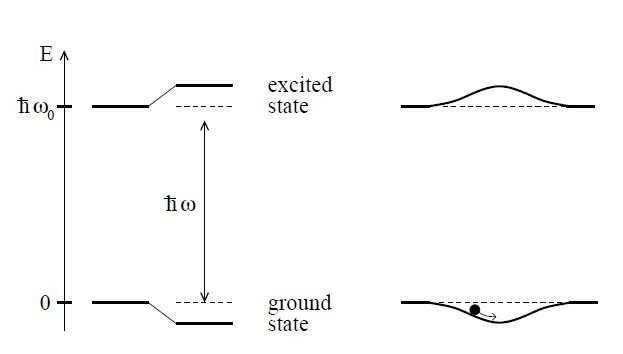
\includegraphics[width=0.5\columnwidth]{Figures/acstark.JPG} 
	\caption{\textit{Light shifts of a two-level atom. Left-hand side,
		red-detuned light ($\Delta < 0$) shifts the ground state down and the
		excited state up by same amounts. Right-hand side, a spatially
		inhomogeneous field like a Gaussian laser beam produces a
		ground-state potential well, in which an atom can be trapped. The figure and 		caption are adopted from \cite{grimm}.}}
	\label{fig:ac_stark} 
\end{figure}
Since the sign is reversed for the excited state, it is important that the atom remains in the ground state. Thus, one has to minimize the scattering with the optical potential. The scattering rate is given as \cite{grimm}
\begin{equation}
	\Gamma_{sc} = \frac{3 \pi c^2}{2 \hbar \omega_{0}^3} \left( \frac{\gamma}{\Delta} \right) I \; .
\end{equation}
Therefore, one has to choose a large detuning in order to reduce the scattering rate, however, this comes at the cost of a weaker potential. Hence, a large intensity must be used to compensate the detuning, such the potential can achieve sufficient depth.